\documentclass{beamer}
\usepackage[latin1]{inputenc}
\usepackage[3D]{movie15}
%\usetheme{Antibes}
\usetheme{Warsaw}
%\usetheme{Marburg}
%\usetheme[secheader]{Boadilla}
%\usetheme{default}
%\usetheme{Dresden}
%\usetheme{Madrid}
%\usecolortheme{seahorse}
%\usecolortheme{crane}
%\usecolortheme{albatross}
%\usecolortheme{whale}
\usecolortheme{beaver}

\usefonttheme{structuresmallcapsserif}

\title[Anatomical Features]{Multivariate models of inter-subject anatomical variability}
\author{John Ashburner}
\institute[j.ashburner@ucl.ac.uk]{Wellcome Trust Centre for Neuroimaging,\\
UCL Institute of Neurology,\\
12 Queen Square,\\
London WC1N 3BG,\\
UK.}
\date{}
\begin{document}

\begin{frame}
\titlepage
\end{frame}

\section{Introduction}
    \subsection{Why apply pattern recognition to structural MRI?}
    \subsection{Common ways to represent anatomical features}
    \subsection{No Free Lunch and prior knowledge}
    \subsection{Dimensionality reduction}
        \subsubsection{Curse of dimensionality}  \begin{frame}
\frametitle{Curse of dimensionality}
\begin{center}
{\Huge Large $p$, small $n$.\par}
\end{center}
\end{frame}

\begin{frame}
\frametitle{Nearest-neighbour classification}
\begin{columns}[c]
\column{0.7\textwidth}
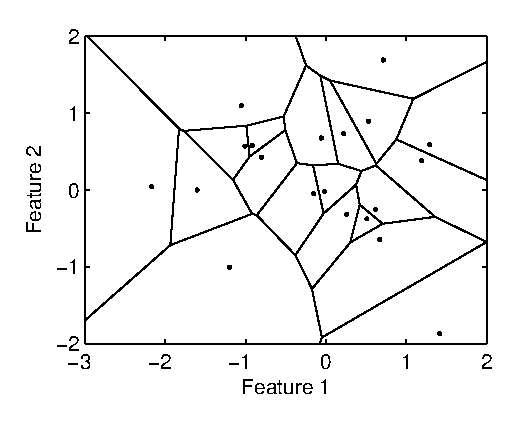
\includegraphics[width=\textwidth]{voronoi}
\column{0.3\textwidth}
\begin{itemize}
\item Not nice smooth separations.
\item Lots of sharp corners.
\item May be improved with \emph{K-nearest neighbours}.
\end{itemize}
\end{columns}
\end{frame}

\begin{frame}
\frametitle{Rule-based approaches}
\begin{columns}[c]
\column{0.7\textwidth}
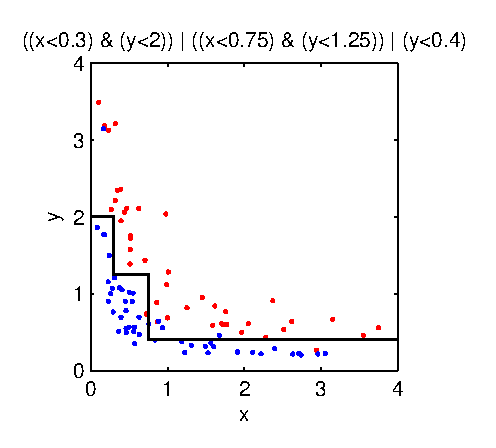
\includegraphics[width=\textwidth]{rule_based}
\column{0.3\textwidth}
\begin{itemize}
\item Not nice smooth separations.
\item Lots of sharp corners.
\end{itemize}
\end{columns}
\end{frame}


\begin{frame}
\frametitle{Corners matter in high-dimensions}
\begin{columns}[c]
\column{0.4\textwidth}
\includegraphics[width=\textwidth]{circle}
\column{0.6\textwidth}
\includegraphics[width=\textwidth]{sphere}
\end{columns}
\end{frame}

\begin{frame}
\frametitle{Corners matter in high-dimensions}
\begin{columns}[c]
\column{0.2\textwidth}
\includegraphics[width=.8\textwidth]{circle}

\includegraphics[width=\textwidth]{sphere}
\column{0.8\textwidth}
\includegraphics[width=\textwidth]{corners}
\end{columns}
\end{frame}

\begin{frame}
\frametitle{Dimensionality $\ne$ number of voxels}
\begin{itemize}
\item Little evidence to suggest that most voxel-based feature selection methods help.
\begin{itemize}
\item Little or no increase in predictive accuracy.
\item Commonly perceived as being more ``interpretable''.
\end{itemize}
\item Prior knowledge derived from independent data is the most reliable way to improve accuracy.
\begin{itemize}
\item e.g. search the literature for clues about which regions to weight more heavily.
\end{itemize}
\end{itemize}

\vspace{1cm}
{\tiny Cuingnet, R\'emi, Emilie Gerardin, J\'er\^ome Tessieras, Guillaume Auzias, St\'ephane Leh\'ericy, Marie-Odile Habert, Marie Chupin, Habib Benali, and Olivier Colliot. ``Automatic classification of patients with Alzheimer's disease from structural MRI: a comparison of ten methods using the ADNI database.'' Neuroimage 56, no. 2 (2011): 766-781.\par}
{\tiny Chu, Carlton, Ai-Ling Hsu, Kun-Hsien Chou, Peter Bandettini, and ChingPo Lin. ``Does feature selection improve classification accuracy? Impact of sample size and feature selection on classification using anatomical magnetic resonance images.'' Neuroimage 60, no. 1 (2012): 59-70.\par}
{\tiny See winning strategies in \url{http://www.ebc.pitt.edu/PBAIC.html}\par}
\end{frame}

\begin{frame}
\frametitle{Linear versus Nonlinear methods}
\begin{columns}[c]
\column{0.7\textwidth}
\begin{itemize}
\item Linear methods are more interpretable.
\item Nonlinear methods usually increase dimensionality.
\item Better to preprocess to obtain features that behave more linearly.
\end{itemize}
\includegraphics[width=\textwidth]{bmi}
\column{0.3\textwidth}
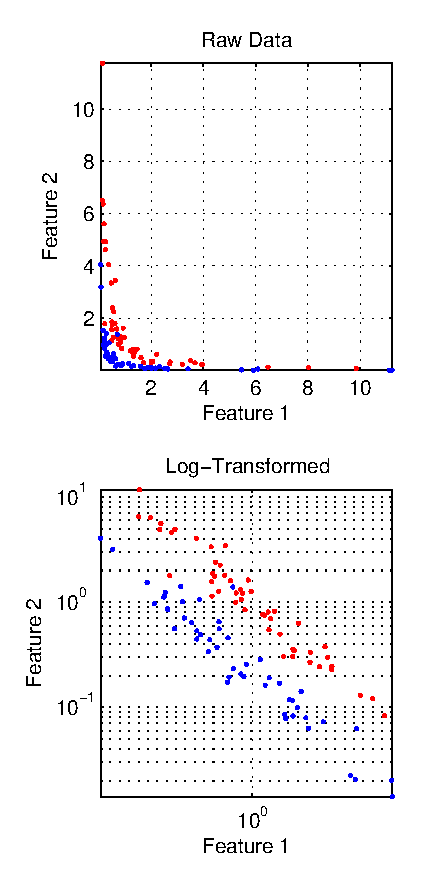
\includegraphics[width=\textwidth]{log_transformed}
\end{columns}
\end{frame}



        \subsubsection{Prediction v Explanation} \begin{frame}
\frametitle{Aims of Science}

\end{frame}


        \subsubsection{Prediction}               \include{Prediction}
        \subsubsection{Binary Classification}    \begin{frame}
\frametitle{A generative classification approach}
\begin{center}
\includegraphics[height=.8\textheight]{fld}
\end{center}
\end{frame}

\begin{frame}
\frametitle{Discriminative classification approaches}
\begin{center}
\includegraphics[height=.8\textheight]{linear_discrimination}
\end{center}
\end{frame}

\begin{frame}
\frametitle{Bayesian classification}
\begin{center}
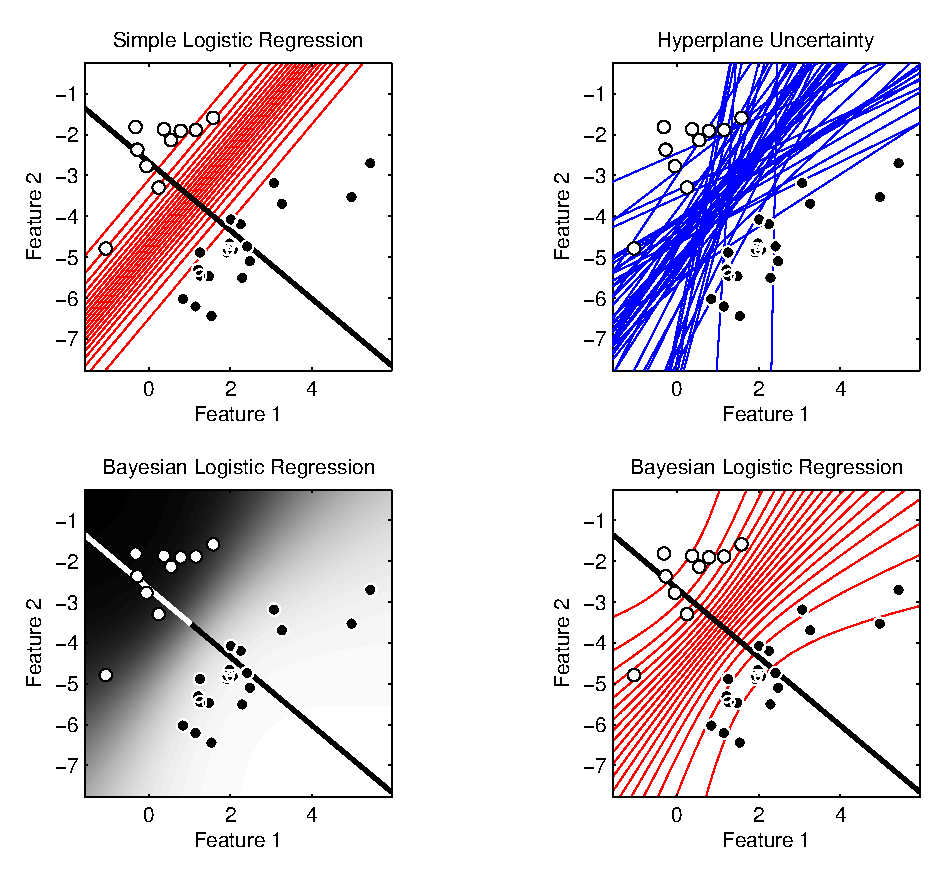
\includegraphics[height=.8\textheight]{logistic_regr}
\end{center}
\end{frame}

\begin{frame}
\frametitle{Why Bayesian?}
\begin{itemize}
\item To deal with different priors.
\begin{itemize}
\item Consider a method with 90\% sensitivity and specificity.
\item Consider using this to screen for a disease afflicting 1\% of the population.
\item On average, out of 100 people there would be 10 wrongly assigned to the disease group.
\item A positive diagnosis suggests only about a 10\% chance of having the disease.
{\small
\begin{eqnarray*}
P(\text{Disease} | \text{Pred+}) & = \frac{P(\text{Pred+} | \text{Disease}) P(\text{Disease})}{P(\text{Pred+} | \text{Disease}) P(\text{Disease}) + P(\text{Pred+} | \text{Healthy}) P(\text{Healthy})}\cr
 & = \frac{\text{Sensitivity} \times P(\text{Disease})}{\text{Sensitivity} \times P(\text{Disease}) + (1-Specificity) \times P(\text{Healthy})}
\end{eqnarray*}
\par
}
\end{itemize}
\item Better decision-making by accounting for utility functions.
\end{itemize}
\end{frame}


        \subsubsection{Kernel methods}           \begin{frame}
\frametitle{There is more than just classification}
\begin{columns}[c]
\column{.4\textwidth}
\begin{itemize}
\item Canonical Correlation Analysis
\item Multi-Way, Multi-View Learning
\item Other existing methods
\item Methods not yet invented
\end{itemize}
\column{.6\textwidth}
\includegraphics[width=\textwidth]{huopaniemi}

{\itshape\tiny Huopaniemi, Ilkka, Tommi Suvitaival, Janne Nikkil\"{a}, Matej Ore\v{s}i\v{c}, and Samuel Kaski. ``Multi-way, multi-view learning.'' arXiv preprint arXiv:0912.3211 (2009).\par}
\end{columns}
\end{frame}


\begin{frame}
\frametitle{Kernel Matrices}
Linear kernel matrices may computed from the raw features.
\begin{eqnarray*}
{\bf C} = {\bf V}{\bf V}^T
\end{eqnarray*}
A simple spatial feature selection may be considered as the following, where ${\bf A}$ is a diagonal matrix of ones and zeros:
\begin{eqnarray*}
{\bf C} = {\bf V}{\bf A}{\bf V}^T
\end{eqnarray*}
However, ${\bf A}$ may be more complicated, for example encoding spatial smoothing, high-pass filtering or any number of other things.
\end{frame}

\begin{frame}
\frametitle{Inner Products}
This gives us an alternative way of measuring distances between vectors in a linear way, where ${\bf A}$ is symmetric and positive definite.
\begin{eqnarray*}
d({\bf v}_1,{\bf v}_2) = \sqrt{({\bf v}_1 - {\bf v}_2)^T {\bf A} ({\bf v}_1 - {\bf v}_2)}
\end{eqnarray*}

Usually, the operation ${\bf A}{\bf v}^T$ is performed as a convolution.  For example, when dealing with 2D data, we may convolve with the Laplacian operator.
\begin{eqnarray*}
{\nabla}^2 {\bf v} = {\bf v} \ast \begin{pmatrix} 0 & -1 & 0\cr -1 & 4 & -1\cr 0 & -1 & 0\end{pmatrix}
\end{eqnarray*}

Note that the actual form of ${\bf A}$ can vary, so we need to figure out what metric tensor is optimal.
\end{frame}



\section{Geometric Morphometrics}
    \subsection{Early univariate morphometry}
    \subsection{Early multivariate morphometry}
    \subsection{The morphometrics ``revolution'' (landmarks)}
    \subsection{Allometric relations}
    \subsection{Automated shape estimation}

    %\subsection{Geometric Variability}
        \subsubsection{Principal Components}     \begin{frame}
\frametitle{One mode of geometric variability}
\begin{columns}[c]
\column{0.5\textwidth}
Simulated images\par
\includegraphics[height=0.9\textwidth]{circles}
\column{0.5\textwidth}
Principal components\par
\includegraphics[height=0.9\textwidth]{circles_pca}
\end{columns}
A suitable model would reduce these data to a single dimension.
\end{frame}


\begin{frame}
\frametitle{Two modes of geometric variability}
\begin{columns}[c]
\column{0.5\textwidth}
Simulated images\par
\includegraphics[height=0.9\textwidth]{things}
\column{0.5\textwidth}
Principal components\par
\includegraphics[height=0.9\textwidth]{things_pca}
\end{columns}
A suitable model would reduce these data to two dimensions.
\end{frame}



\section{Similarity between brains}
    \subsection{Distances between anatomies} \begin{frame}
\frametitle{Similarity Measures}
\begin{itemize}
\item Many methods are based on similarity measures.
\item A common similarity measure is the dot product.
\begin{eqnarray*}
\text{Similarity: } k({\bf x},{\bf y}) = \sum_k x_k y_k
\end{eqnarray*}
\item Nonlinear methods are often based on distances.
\begin{eqnarray*}
\text{Distance: } & d({\bf x},{\bf y}) = & \sqrt{\sum_k (x_k-y_k)^2}\cr
\text{Similarity: } & k({\bf x},{\bf y}) = & exp(-\lambda d({\bf x},{\bf y})^2)
\end{eqnarray*}
\item How do we best measure distances between brain images?
\end{itemize}
\end{frame}

%\begin{frame}
%\frametitle{No Free Ducklings}
%{\bf No Free Lunch theorem} says that learning is impossible without prior knowledge (\url{http://en.wikipedia.org/wiki/No\_free\_lunch\_in\_search\_and\_optimization}).

%{\bf Ugly Duckling theorem} says that things are all equivalently similar to each other without prior knowledge (\url{http://en.wikipedia.org/wiki/Ugly\_duckling\_theorem}).

%\vspace{1cm}
%What prior knowledge do we have about the variability among people that can be measured using MRI?

%How do we use this knowledge?
%\end{frame}

\begin{frame}
\frametitle{Image Registration}
\begin{columns}[c]
\column{0.7\textwidth}
\begin{itemize}
\item Image registration measures distances between images.
\item Often involves minimising the sum of two terms:
\begin{itemize}
\item Distance between the image intensities.
\item Distance of the deformation from zero.
\end{itemize}
\item The sum of these terms gives the distance.
\end{itemize}
\column{0.3\textwidth}
\includegraphics[width=\textwidth]{shoot2d}
\end{columns}
\end{frame}

\begin{frame}
\frametitle{Different ways of measuring distances}
\begin{columns}[c]
\column{.3\textwidth}
\includegraphics[width=\textwidth]{mumford}
\column{.7\textwidth}
\includegraphics[width=\textwidth]{mumford_fig}
\end{columns}
\end{frame}

\begin{frame}
\frametitle{Different ways of measuring distances}
\begin{columns}[c]
\column{.2\textwidth}
\begin{center}
Two simulated images\par
\includegraphics[width=\textwidth]{figure2Di}
\end{center}
\column{.8\textwidth}
\includegraphics[width=\textwidth]{figure2Dii}
\end{columns}
\end{frame}

\begin{frame}
\frametitle{Metrics}
Distances need to satisfy the properties of a \emph{metric}:
\begin{enumerate}
\item $d({\bf x}, {\bf y}) \ge 0$ (non-negativity)
\item $d({\bf x}, {\bf y}) = 0$ if and only if ${\bf x} = {\bf y}$ (identity of indiscernibles)
\item $d({\bf x}, {\bf y}) = d({\bf y}, {\bf x})$ (symmetry)
\item $d({\bf x}, {\bf z}) \le d({\bf x}, {\bf y}) + d({\bf y}, {\bf z})$ (triangle inequality).
\end{enumerate}

Satisfying (3) requires inverse-consistent image registration.

Satisfying (4) requires a specific class of image registration models.
\end{frame}


\begin{frame}
\frametitle{Non-Euclidean geometry}
\begin{columns}[c]
\column{0.5\textwidth}
\begin{itemize}
\item Distances are not always measured along a straight line.
\item ``\emph{Shapes are the ultimate non-linear sort of thing}''
\end{itemize}
\column{0.5\textwidth}
\includegraphics[width=\textwidth]{Globe}
\end{columns}
\end{frame}

\begin{frame}
\frametitle{Linear approximations to nonlinear problems}
%\begin{columns}[c]
%\column{0.2\textwidth}
%Dealing with non-Euclidean geometry.
%Linear approximation around the average.
%\begin{center}
%\column{0.8\textwidth}
\begin{center}
\includegraphics[width=1.2\textwidth]{spheres}
\end{center}
%\end{columns}
\end{frame}

%\begin{frame}
%\frametitle{D'Arcy Thompson's Generative Model}
%\begin{quote}
%``...diverse and dissimilar fishes can be referred as a whole to identical functions of very different co-ordinate systems...''
%\end{quote}
%\begin{center}
%\includegraphics[height=0.4\textheight]{OGAF}
%\includegraphics[height=0.4\textheight]{fish}
%\end{center}
%We can compute relative shapes using image registration.
%\end{frame}


    \subsection{Non-linear distances (manifolds)}
        \subsubsection{Manifolds}                \include{Manifolds}

    \subsection{Image registration for measuring distances}
    \subsection{Tangent space representations}
    \subsection{Scalar momenta}
    \subsection{Empirical examples}
        \subsubsection{Data}                     \begin{frame}
\frametitle{Real data}
\begin{columns}[c]
\column{0.5\textwidth}
Used 550 T1w brain MRI from IXI ({\bf I}nformation e{\bf X}traction from {\bf I}mages) dataset.

\url{http://www.brain-development.org/}

Data from three different hospitals in London:
\begin{itemize}
\item{Hammersmith Hospital using a Philips 3T system}
\item{Guy's Hospital using a Philips 1.5T system}
\item{Institute of Psychiatry using a GE 1.5T system}
\end{itemize}

\column{0.5\textwidth}
\includegraphics[width=0.9\textwidth]{orig_ixi}
\end{columns}
\end{frame}

\begin{frame}
\frametitle{Grey and White Matter}
\begin{columns}[c]
\column{0.26\textwidth}
Segmented into GM and WM.

Approximately aligned via rigid-body.
\column{0.75\textwidth}
\includegraphics[width=0.5\textwidth]{gm_ixi}
\includegraphics[width=0.5\textwidth]{wm_ixi}
\end{columns}

\begin{tiny}
Ashburner, J \& Friston, KJ. \emph{Unified segmentation}. NeuroImage 26(3):839--851 (2005).

\end{tiny}
\end{frame}

\begin{frame}
\frametitle{Diffeomorphic Alignment}
All GM and WM were diffeomorphically aligned to their common average-shaped template.
\begin{center}
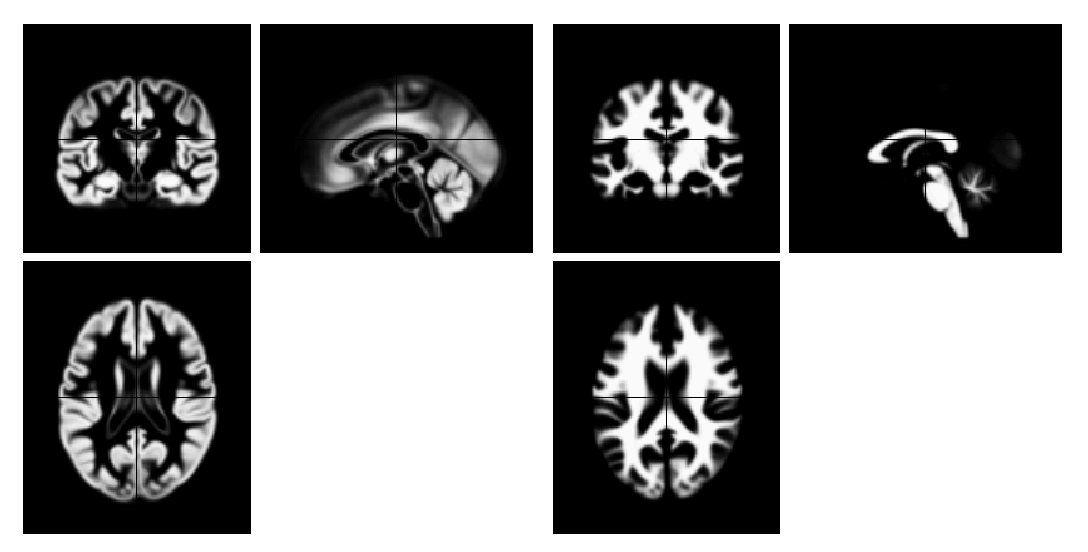
\includegraphics[width=.8\textwidth]{template}
\end{center}

\begin{tiny}
Ashburner, J \& Friston, KJ. \emph{Diffeomorphic registration using geodesic shooting and Gauss-Newton optimisation}. NeuroImage 55(3):954--967 (2011).

Ashburner, J \& Friston, KJ. \emph{Computing average shaped tissue probability templates}. NeuroImage 45(2):333--341 (2009).

\end{tiny}
\end{frame}


        \subsubsection{Features}                 \begin{frame}
\frametitle{Volumetric Features}
\begin{columns}[c]
\column{0.33\textwidth}
A number of features were used for pattern recognition.

Firstly, two features relating to relative volumes.

Initial velocity divergence is similar to logarithms of Jacobian determinants.
\column{0.33\textwidth}
Jacobian Determinants

\includegraphics[width=1\textwidth]{jac_ixi}
\column{0.33\textwidth}
Initial Velocity Divergence
\includegraphics[width=1\textwidth]{div_ixi}
\end{columns}
\end{frame}

%%%%%%%%%%%%%%%%%%%%%%%%%%%%%%%%%%%%%%%%%%%%%%%%%%%%%%%%%%%%%%%
\begin{frame}
\frametitle{Grey Matter Features}
\begin{columns}[c]
\column{0.33\textwidth}
Rigidly Registered GM

\includegraphics[width=1\textwidth]{gm_ixi}

\column{0.33\textwidth}
Nonlinearly Registered GM

\includegraphics[width=1\textwidth]{wc1_ixi}
\column{0.33\textwidth}
Registered and Jacobian Scaled GM

\includegraphics[width=1\textwidth]{mwc1_ixi}
\end{columns}
\end{frame}

%%%%%%%%%%%%%%%%%%%%%%%%%%%%%%%%%%%%%%%%%%%%%%%%%%%%%%%%%%%%%%%
%%%%%%%%%%%%%%%%%%%%%%%%%%%%%%%%%%%%%%%%%%%%%%%%%%%%%%%%%%%%%%%
\begin{frame}
\frametitle{``Scalar Momentum'' Features}
\begin{columns}[c]
\column{0.33\textwidth}
``Scalar momentum'' actually has two components because GM was matched with GM and WM was matched with WM.
\column{0.33\textwidth}
First Momentum Component

\includegraphics[width=1\textwidth]{resids1_ixi}
\column{0.33\textwidth}
Second Momentum Component

\includegraphics[width=1\textwidth]{resids2_ixi}
\end{columns}
\end{frame}



        \subsubsection{Results}                  \begin{frame}
\frametitle{Age Regression}
Linear Gaussian Process Regression to predict subject ages.
\begin{columns}[c]
\column{0.5\textwidth}
\includegraphics[width=1\textwidth]{age_loglikelihood}
\column{0.5\textwidth}
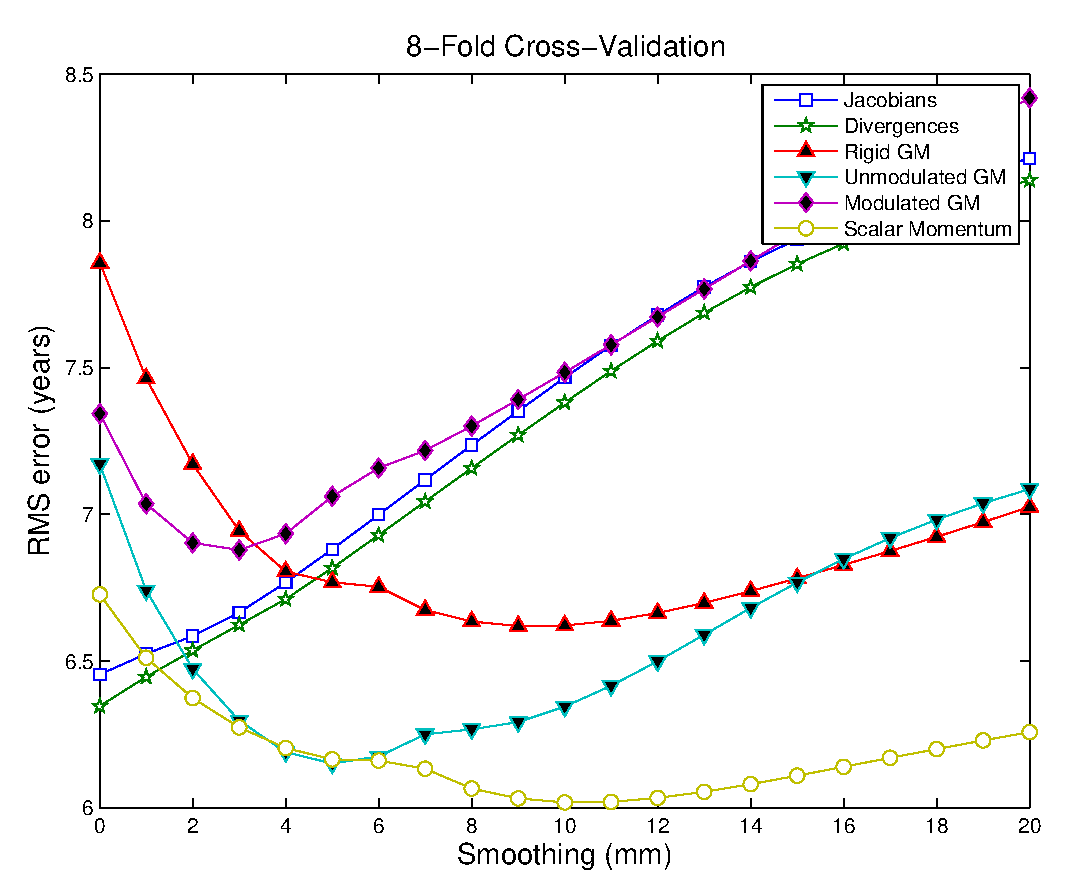
\includegraphics[width=1\textwidth]{age_rms}
\end{columns}

\begin{tiny}
Rasmussen, CE \& Williams, CKI. \emph{Gaussian processes for machine learning}. Springer (2006).

\end{tiny}
\end{frame}

%%%%%%%%%%%%%%%%%%%%%%%%%%%%%%%%%%%%%%%%%%%%%%%%%%%%%%%%%%%%%%%
\begin{frame}
\frametitle{Sex Classification}
Linear Gaussian Process Classification (EP) to predict sexes.
\begin{columns}[c]
\column{0.5\textwidth}
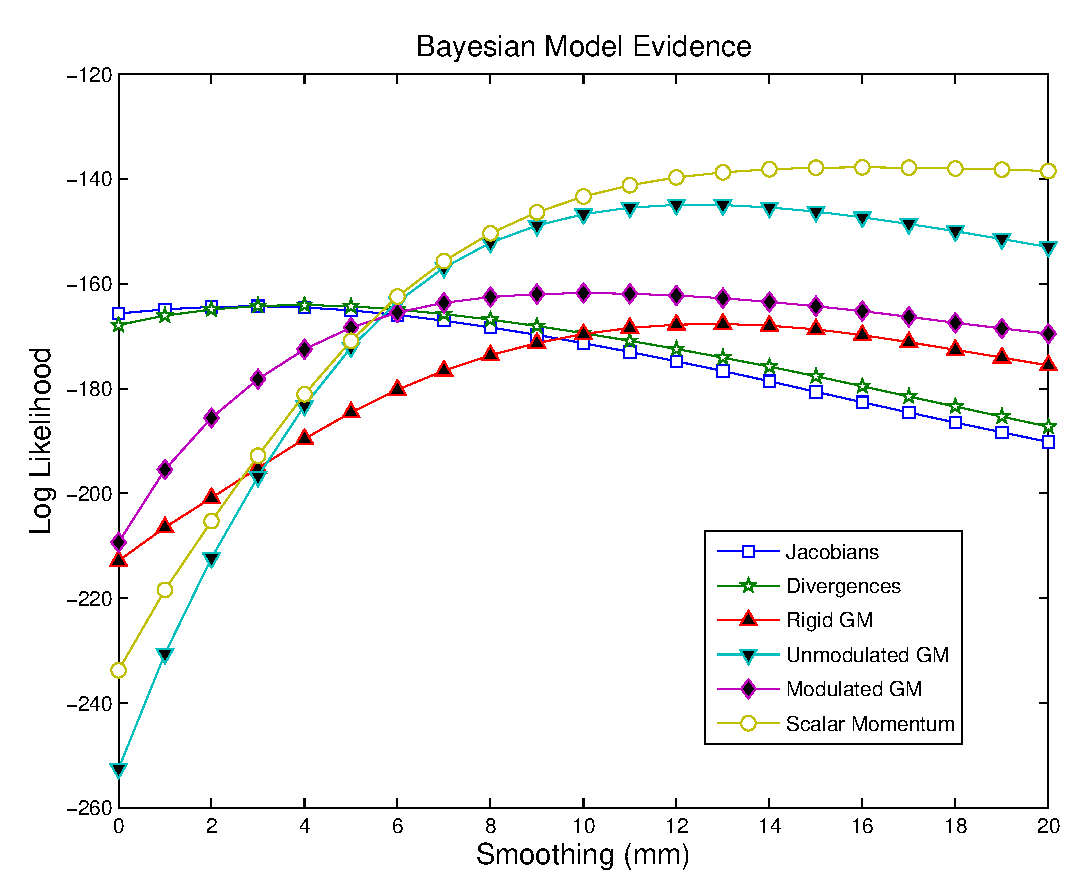
\includegraphics[width=1\textwidth]{sex_loglikelihood}
\column{0.5\textwidth}
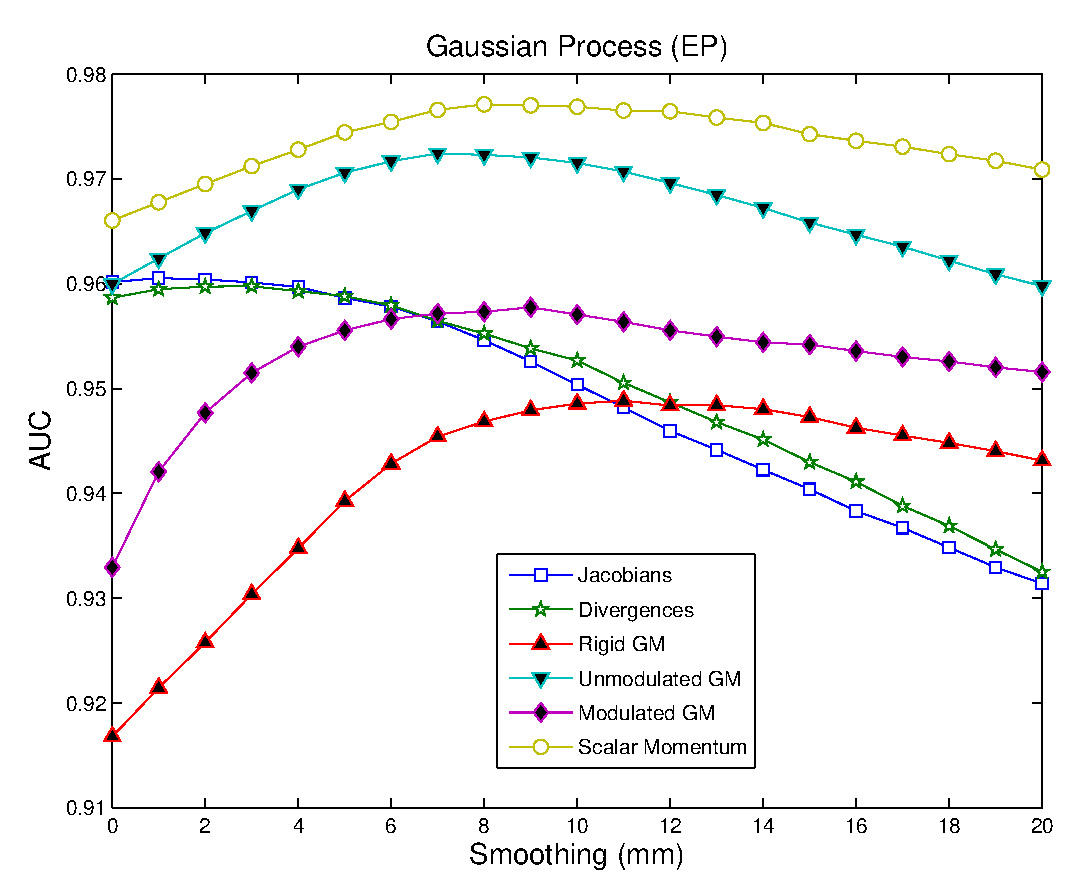
\includegraphics[width=1\textwidth]{sex_auc_GP}
\end{columns}

\begin{tiny}
Rasmussen, CE \& Williams, CKI. \emph{Gaussian processes for machine learning}. Springer (2006).

\end{tiny}
\end{frame}

%%%%%%%%%%%%%%%%%%%%%%%%%%%%%%%%%%%%%%%%%%%%%%%%%%%%%%%%%%%%%%%
%\begin{frame}
%\frametitle{Sex Classification}
%Linear SVM versus Gaussian Process Classification (EP).
%\begin{columns}[c]
%\column{0.5\textwidth}
%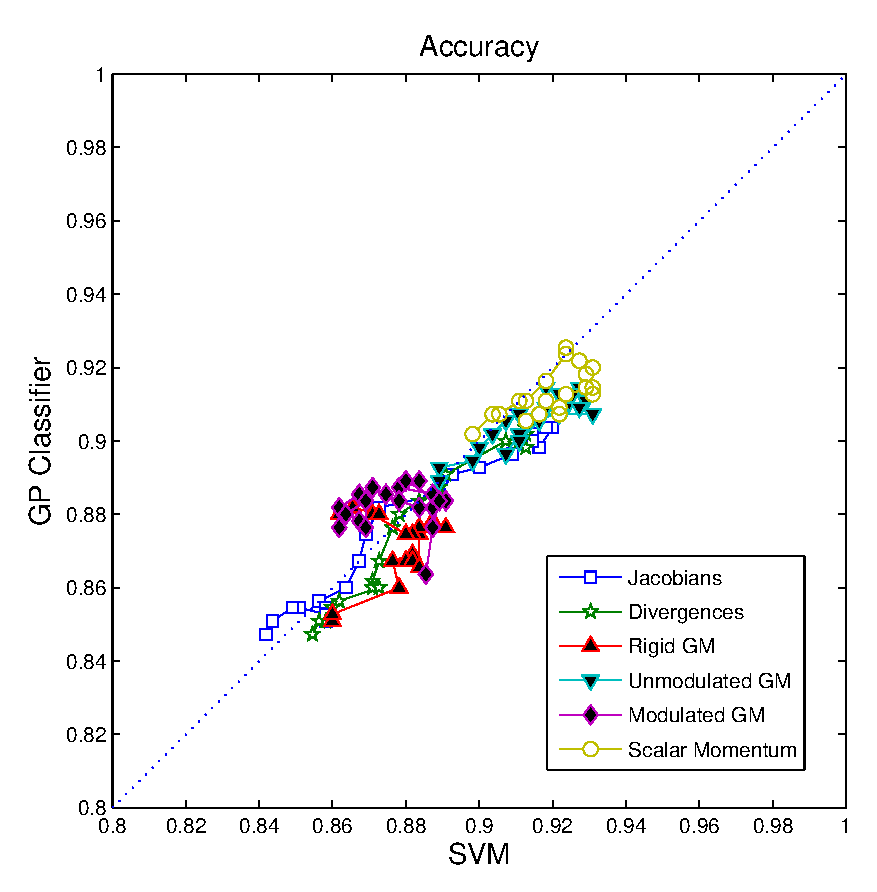
\includegraphics[width=1\textwidth]{sex_SVM_v_GP_acc}
%\column{0.5\textwidth}
%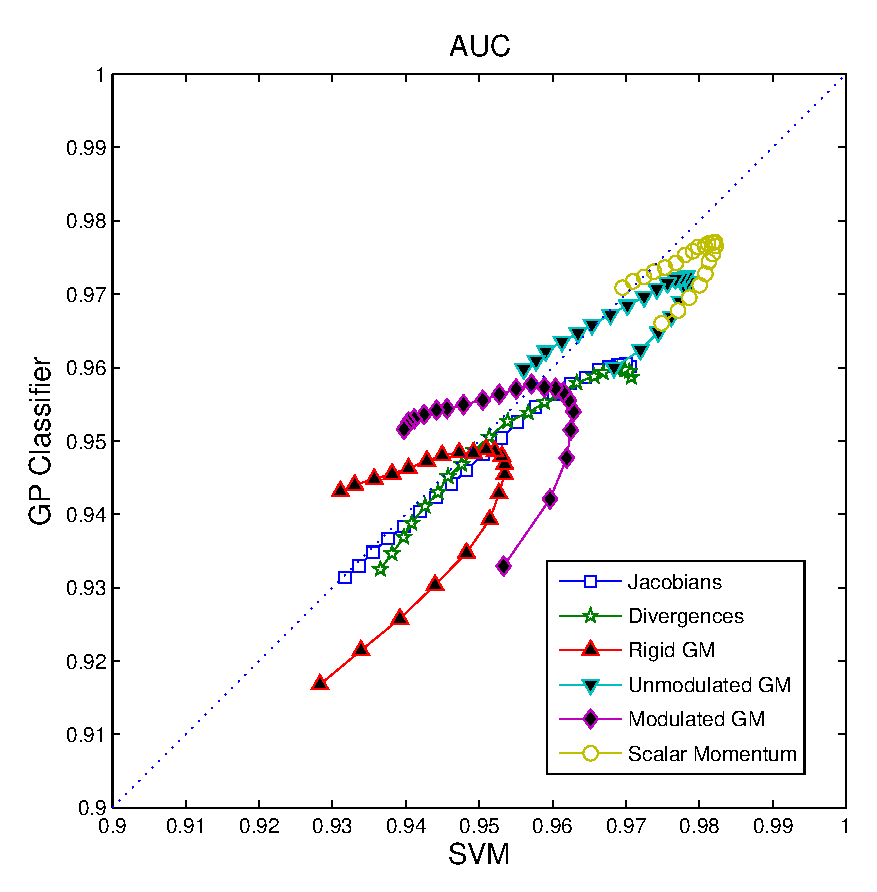
\includegraphics[width=1\textwidth]{sex_SVM_v_GP_AUC}
%\end{columns}
%\end{frame}

%%%%%%%%%%%%%%%%%%%%%%%%%%%%%%%%%%%%%%%%%%%%%%%%%%%%%%%%%%%%%%%

\begin{frame}
\frametitle{Predictive Accuracies}
\begin{columns}[c]
\column{0.5\textwidth}

Age

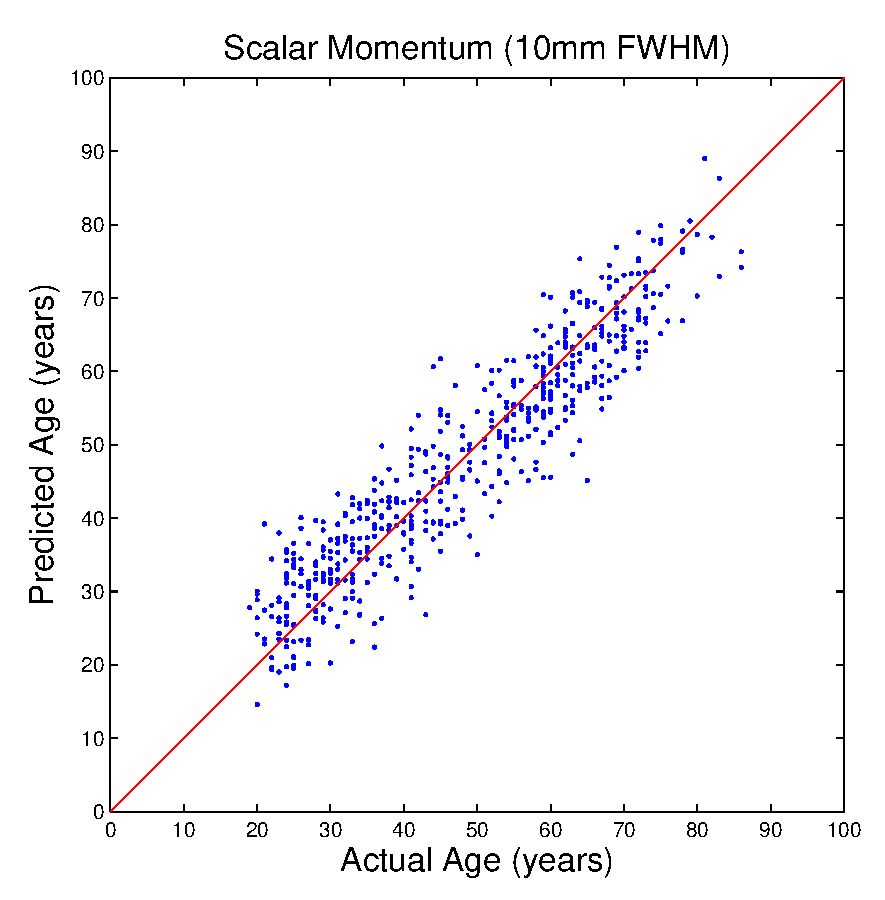
\includegraphics[width=1\textwidth]{age_predictions}
\column{0.5\textwidth}

Sex

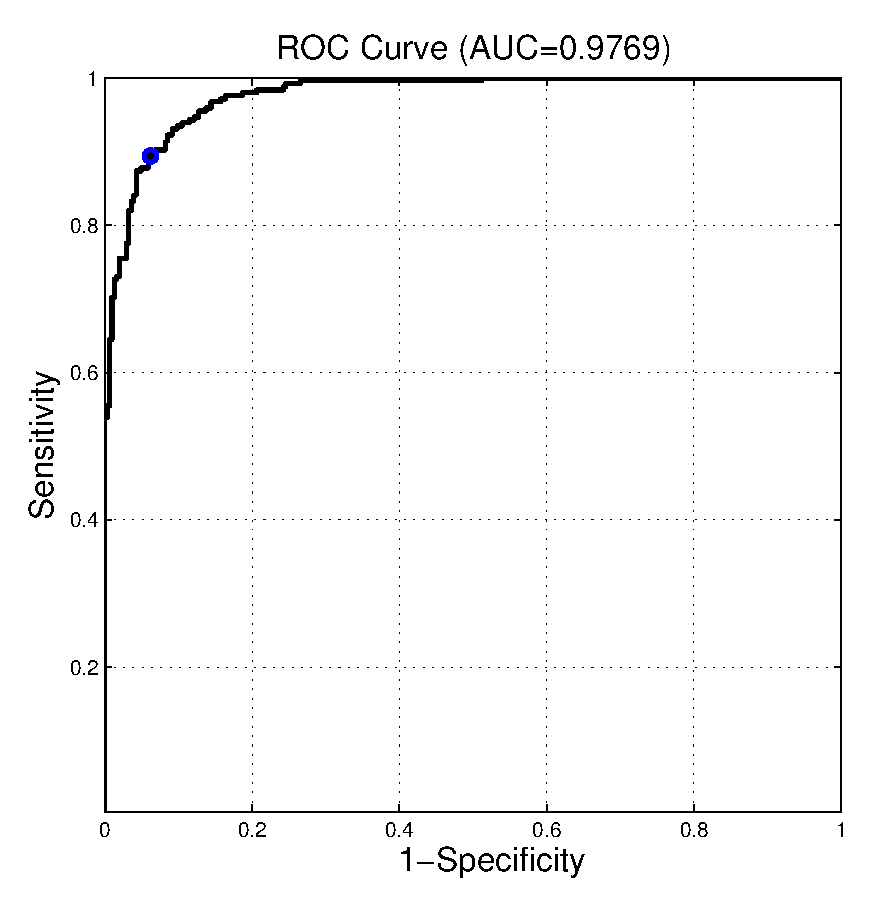
\includegraphics[width=1\textwidth]{sex_roc}
\end{columns}
\end{frame}

\begin{frame}
\frametitle{Conclusions}
\begin{itemize}
\item{Scalar momentum (with about 10mm smoothing) appears to be a useful feature set.}
\item{Jacobian-scaled warped GM is surprisingly poor.}
%\item{SVC slightly more accurate than GP (but we knew that already).}
\item{Amount of spatial smoothing makes a big difference.}
\item{Further dependencies on the details of the registration still need exploring.}
\end{itemize}
\end{frame}
%%%%%%%%%%%%%%%%%%%%%%%%%%%%%%%%%%%%%%%%%%%%%%%%%%%%%%%%%%%%%%%
%\begin{frame}
%\frametitle{Additional references}
%\begin{itemize}
%\item{Ashburner, J \& Kl\"oppel, K. \emph{Multivariate models of inter-subject anatomical variability}. NeuroImage 56(2):422--439 (2011).}
%\item{Ashburner, J \& Friston, KJ. \emph{Diffeomorphic registration using geodesic shooting and Gauss-Newton optimisation}. NeuroImage 55(3):954--967 (2011).}
%\end{itemize}
%\end{frame}

\begin{frame}
\begin{center}
\includegraphics[width=.8\textwidth]{hyper_male}
\end{center}
\end{frame}

\begin{frame}
\begin{center}
\includegraphics[width=.8\textwidth]{avgT1}
\end{center}
\end{frame}

\begin{frame}
\begin{center}
\includegraphics[width=.8\textwidth]{hyper_female}
\end{center}
\end{frame}




%    \subsection{Examples of features}     \begin{frame}
\frametitle{Example Images}
Some example (non-brain) images.
\begin{center}
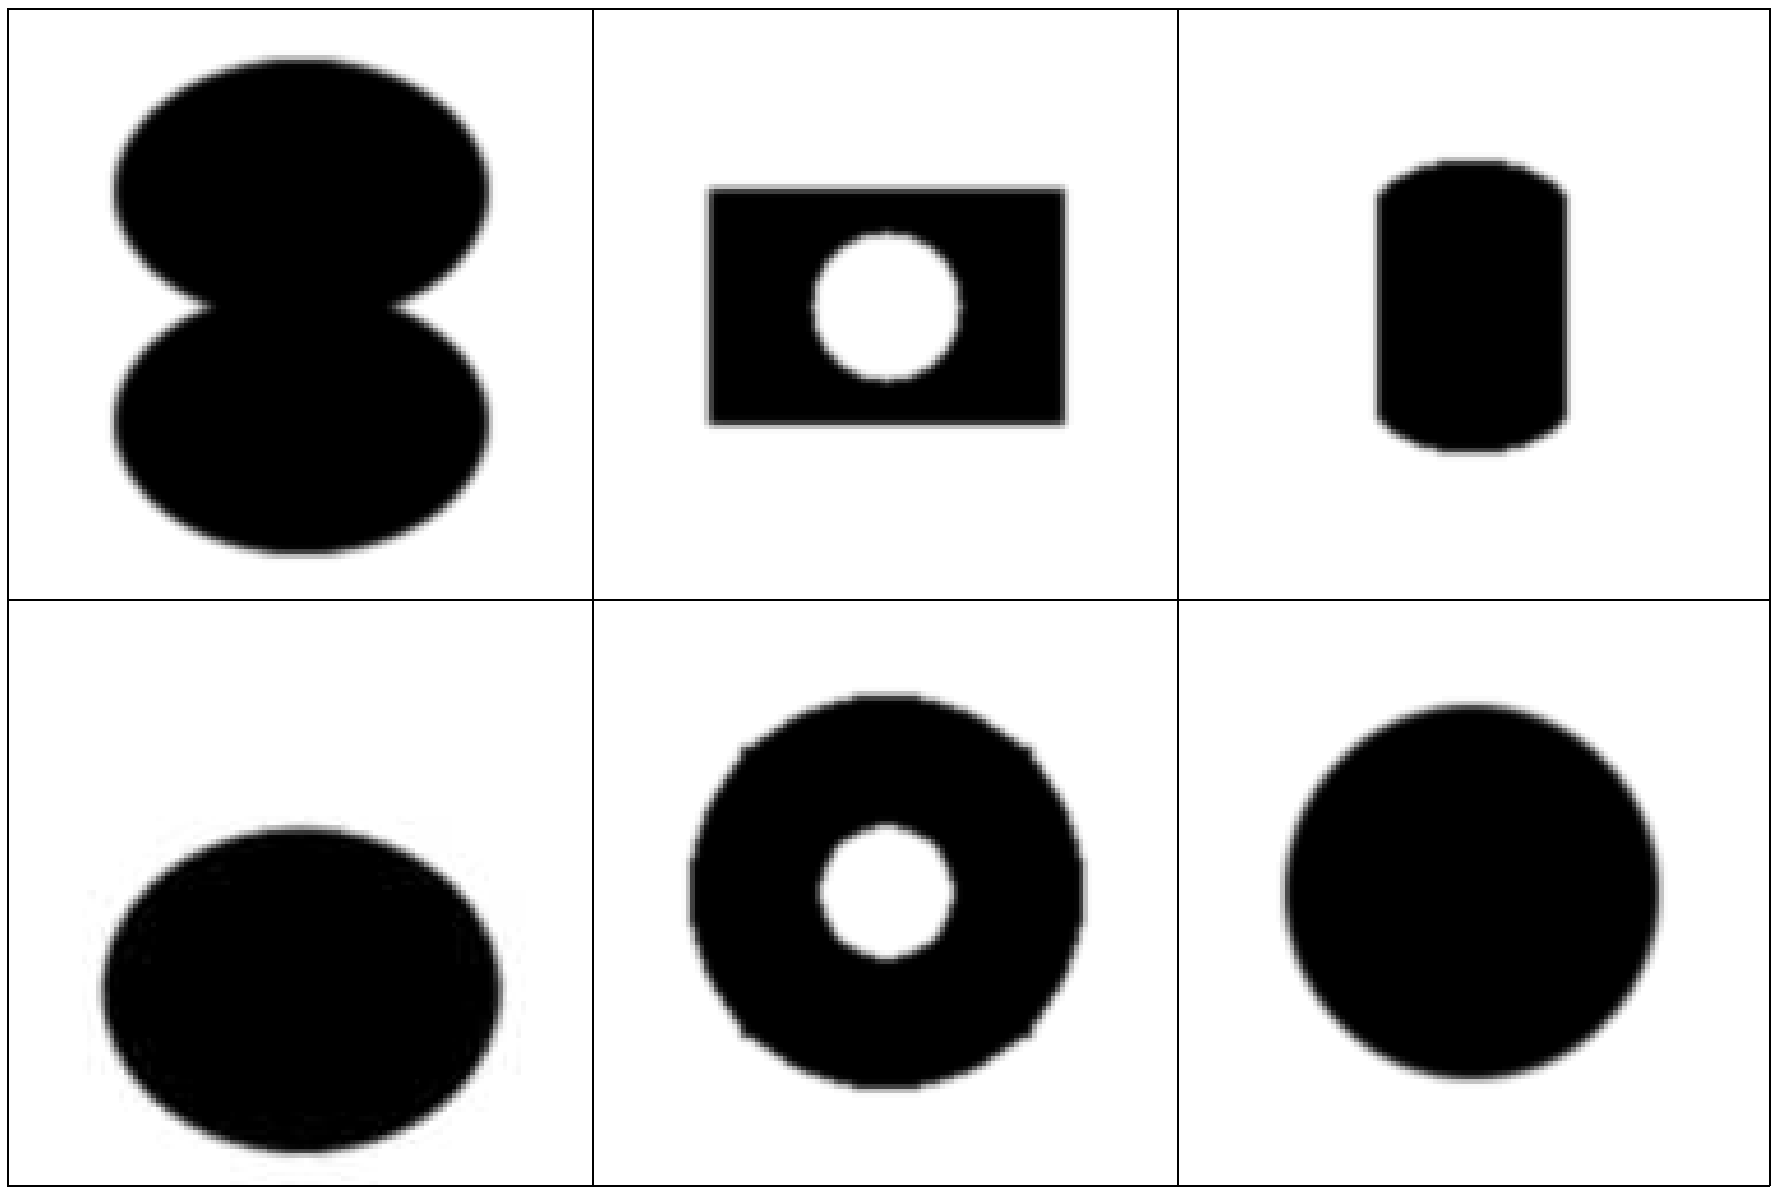
\includegraphics[width=0.9\textwidth]{original}
\end{center}
\end{frame}

%\begin{frame}
%\frametitle{Samples from a Linear Generative Model}
%Did the images come from a model like this?
%\begin{center}
%\includegraphics[width=0.9\textwidth]{simulated_lin}
%\end{center}
%\end{frame}

%\begin{frame}
%\frametitle{Samples from a Geometric Generative Model}
%Or one like this?
%\begin{center}
%\includegraphics[width=0.9\textwidth]{simulated}
%\end{center}
%\end{frame}

\begin{frame}
\frametitle{Registered Images}
We could register the images to their average shape...
\begin{center}
\includegraphics[width=0.9\textwidth]{warped}
\end{center}
\end{frame}

\begin{frame}
\frametitle{Deformations}
...and study the deformations...
\begin{center}
\includegraphics[width=0.9\textwidth]{deformations}
\end{center}
\end{frame}

\begin{frame}
\frametitle{Jacobian Determinants}
...or the relative volumes...
\begin{center}
\includegraphics[width=0.9\textwidth]{jacobians}
\end{center}
\end{frame}

\begin{frame}
\frametitle{Scalar Momentum}
... or ``scalar momentum'' (Singh et al, MICCAI 2010).
\begin{center}
\includegraphics[width=0.9\textwidth]{alpha}
\end{center}
\end{frame}

\begin{frame}
\frametitle{Reconstructed Images}
Reconstructions from template and scalar momenta.
\begin{center}
\includegraphics[width=0.9\textwidth]{reconstructed}
\end{center}
\end{frame}

%\begin{frame}
%\frametitle{Evolution}
%\begin{center}
%\includegraphics[width=.8\textwidth]{evolution}\par
%\begin{tiny}
%Singh, Fletcher, Preston, Ha, King, Marron, Wiener \& Joshi (2010). \emph{Multivariate Statistical Analysis of Deformation Momenta Relating Anatomical Shape to Neuropsychological Measures}. T. Jiang et al. (Eds.): MICCAI 2010, Part III, LNCS 6363, pp. 529--537, 2010.\par
%\end{tiny}
%\end{center}
%\end{frame}



\section{Conclusion: What next?}

\end{document}
